\documentclass[a4paper]{article}

\usepackage[T1]{fontenc}
%\usepackage[utf8]{inputenc}
\usepackage[brazil]{babel}

\usepackage{verbatim}
\usepackage{geometry}
\usepackage{hyperref}
\usepackage{fontspec}
\usepackage{fancyhdr}


\usepackage{parskip}
\setlength{\parskip}{1em}

\usepackage{minted}

% Define um ambiente personalizado
%\newenvironment{myMinted}[1] {\begin{minted}[frame=single, fontsize=\small, baselinestretch=1.2]{#1}\vspace{-1em}} {\end{minted}\vspace{-1em}}  



\usepackage{amsmath, amssymb, amsfonts}
\usepackage{mathtools}
\usepackage{graphicx}
\usepackage{physics}
\usepackage{siunitx}

\title{Resumo \\ Introdução à Utilização de \\  \textbf{\huge Git \& Github}}
\author{Hygor Melo de Sena}
\date{11 de janeiro de 2026}

\sloppy

\setmainfont{Spectral}



%\setcounter{secnumdepth}{0}

\hypersetup{
    colorlinks=true,
    linkcolor=blue,      
    linktoc=all          
}

\pagestyle{fancy}



\begin{document}
    \maketitle
    
    \newpage
    
    \tableofcontents
    
    \newpage
    
    \section{Capítulo 1 $ \blacktriangleright $ O que é Git? O que é versionamento?}
    
    \bigskip
    
    Git é um dos sistemas de controle de versões de programas, ou seja, ele é um sistema de controle de versão (\textit{VCS}). Dessa afirmação tiramos o significado de versionamento. Versionamento trata-se simplesmente de versões que um \textit{software} pode sofrer durante seu processo de desenvolvimento como se pode ver abaixo:
    
    \medskip
    
    \begin{figure}[hb] % Parâmetros de posição
        \centering % Centralizando imagem na posição
        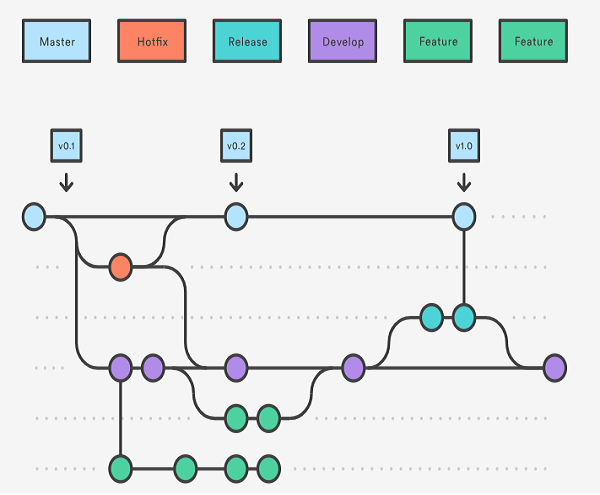
\includegraphics[scale=0.6]{./imagens/gitglow.png} % Inserindo imagem redimensionada
        \caption{Fluxograma de Versionamento Git} % Legenda da imagem
    \end{figure}   	
    
    \medskip
    
    Na figura acima também podemo ver o ciclo de versionamento do Git. Temos a versão Master, Hotfix, Develop, Release, Feature. Master tem por finalidade um branch de produção, Develop é branch de integração contínua do desenvolvimento, Feature é desenvolvimento de novas funcionalidades específicas, Realese é preparar uma versão candidata à produção, Hotfix é correção urgente em produção. Confira a tabela abaixo:
    
    \bigskip
    
    \begin{center}
        \begin{tabular}{l r r r r}
            \hline 
            Branch & Objetivo Principal & Estável & Origem & Destino Final\\
            \hline
            Master & Produção & Sim & Release/Hotfix & —\\
            \hline
            Develop & Integração do desenvolvimento & Parcial & Master & Release\\
            \hline
            Feature & Nova funcionalidade & Não & Develop & Develop\\
            \hline
            Release & Estabilização de versão & Quase & Develop & Master + Develop\\
            \hline
            Hotfix & Correção urgente & Sim & Master & Master + Develop\\
        \end{tabular}
    \end{center}
    
    \newpage
    
    \section{Capítulo 2 $ \blacktriangleright $ O que é GitHub? Para que serve?}
    
    \bigskip
    
    \textbf{GitHub} é uma plataforma online de hospedagem e colaboração de código baseada no Git, utilizada para versionar, compartilhar, revisar e gerenciar projetos de software de forma organizada e rastreável.
    \smallskip
    Em termos práticos, o GitHub permite:
    
    \begin{itemize}
        \item Armazenar código-fonte em repositórios remotos.
        \item Controlar versões (histórico completo de alterações).
        \item Trabalhar em equipe, com múltiplas pessoas atuando no mesmo projeto sem sobrescrever código.
        \item Criar e revisar mudanças por meio de \textit{branches}, \textit{commits} e \textit{pull requests}.
        \item Documentar projetos (README, wikis).
        \item Automatizar processos com CI/CD (Github Actions)
        \item Gerenciar tarefas com \textit{issues}, \textit{milestones} e projetos.
    \end{itemize}	
    
    \medskip
    
    Em uma frase: GitHub é o ambiente onde projetos versionados com Git vivem, evoluem e são colaborados publicamente ou de forma privada.
    
    \newpage
    
    \section{Capítulo 3 $ \blacktriangleright $ A evolução do Git e GitHub}
    
    Git (2005) nasceu da necessidade e da raiva:\\
    Linus Torvalds ficou sem ferramenta boa depois da briga com a BitKeeper, criou algo rápido, poderoso, distribuído e com integridade de dados fortíssima.
    
    GitHub (2008) nasceu da pergunta:\\
    "E se a gente pegasse esse Git incrível... e colocasse uma interface web bonita + rede social + colaboração fácil em cima dele?"
    
    Resultado:
    GitHub transformou o Git de "ferramenta de linha de comando para nerds do kernel" em algo que todo mundo usa (empresas, iniciantes, open-source, times enormes, educação...).
    Curiosidades legais
    O primeiro commit do Git (7 de abril de 2005) foi um README bem simples
    O apelido inicial do Git dado pelo próprio Linus: "the information manager from hell".\\ 
    GitHub demorou alguns anos para ficar famoso, mas quando explodiu... foi muito rápido
    Hoje em dia muita gente fala "Git" quando na verdade quer dizer "GitHub" (e vice-versa)
    Resumindo em uma frase:
    Git resolveu o problema técnico de controle de versão distribuído.
    GitHub resolveu o problema social de como milhões de programadores trabalham juntos.
    
    
    \newpage
    
    \section{Capítulo 4 $ \blacktriangleright $ Instalações e configurações importantes}
    
    \newpage
    
    \section{Capítulo 5 $ \blacktriangleright $ Clonando um Repositório}
    
    A clonagem de repositórios do GitHub é essencial para que se possa trabalhar com o código fonte de terceiro ou projeto de terceiro facilmente. E o processo é simples como se pode ver abaixo:
    
    \medskip
    
    \begin{figure}[hb]
        \centering
        \includegraphics*[scale=0.4]{./imagens/githubclonetest.png}
        \caption{Exemplo de clonagem de repositório}
    \end{figure}
    
    \medskip
    
    Como mostra a imagem acima, é possivel clonar repositório de forma simples com o github desktop (ferramenta facilitadora). Deve-se observar que o repositório clonado de terceiro não pode ser alterado e enviado como uma modificação original, ou seja, o repositório clonado pode ser usado apenas para testes e projetos pessoais observando a licença daquele. O que pode ser feito é sugerir modificações para o dono do repositório e/ou iniciar uma \textit{fork}. Como podemos ver nessa outra imagem abaixo a modificação do diretório associado a clonagem do \textit{repo} do prof. Guanabara não pode ser "subida" de modo a substitui o original.
    
   
    
    \begin{figure}[h!]
        \centering
        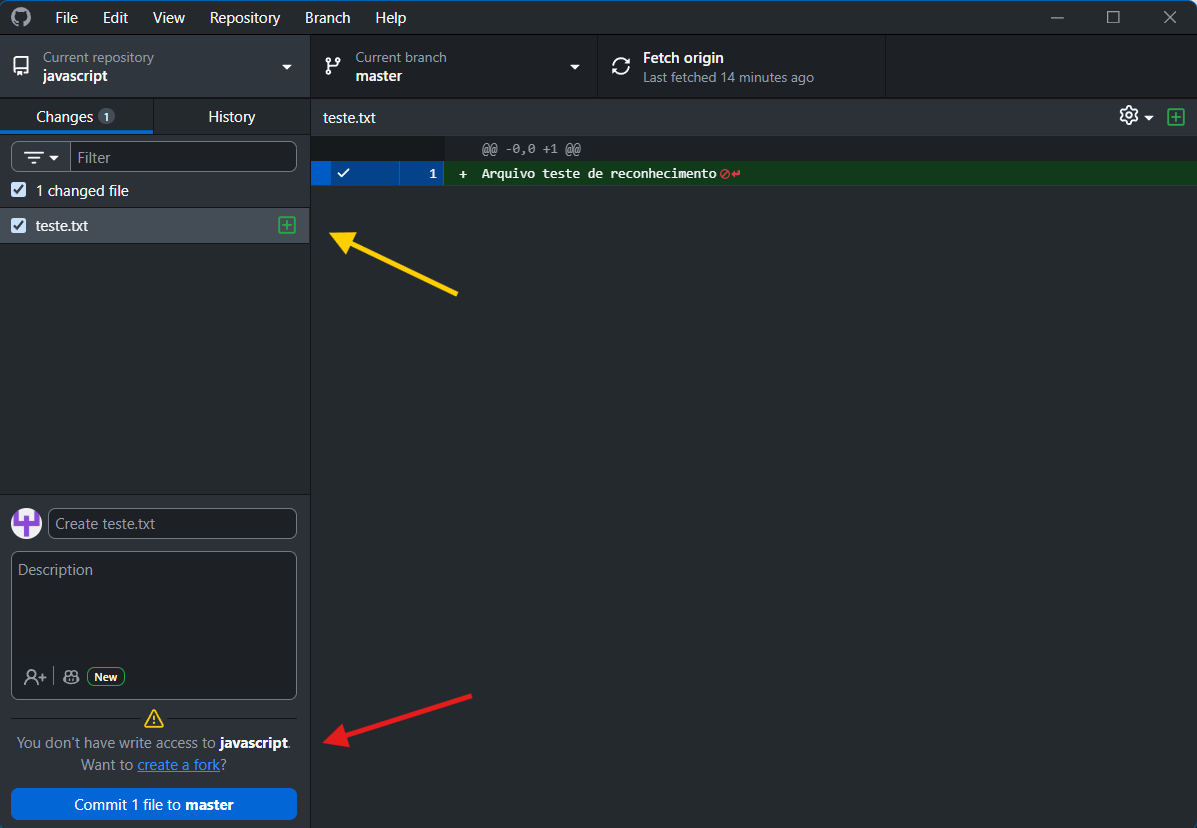
\includegraphics[scale=0.5]{./imagens/testsdemodificacaorepoterceiro.png}
        \caption{Exemplo de modificação de \textit{repo} de terceiro.}
    \end{figure} 
    
    
    \newpage
    
    \section{Capítulo 6 $ \blacktriangleright $ Versionando seus projetos antigos}

    O versionamento de um é feito de forma automática pelo \textbf{GitHub-Desktop} todas as vezes que se faz um \textit{commit} na \textit{branch-master} ou demais \textit{branchs} como vimos no capitulo 1. Cada \textit{commit} salva o estado do seu projeto com as modificações feitas. Podemos observar isso abaixo:
    
    \begin{figure}[h!]
        \centering
        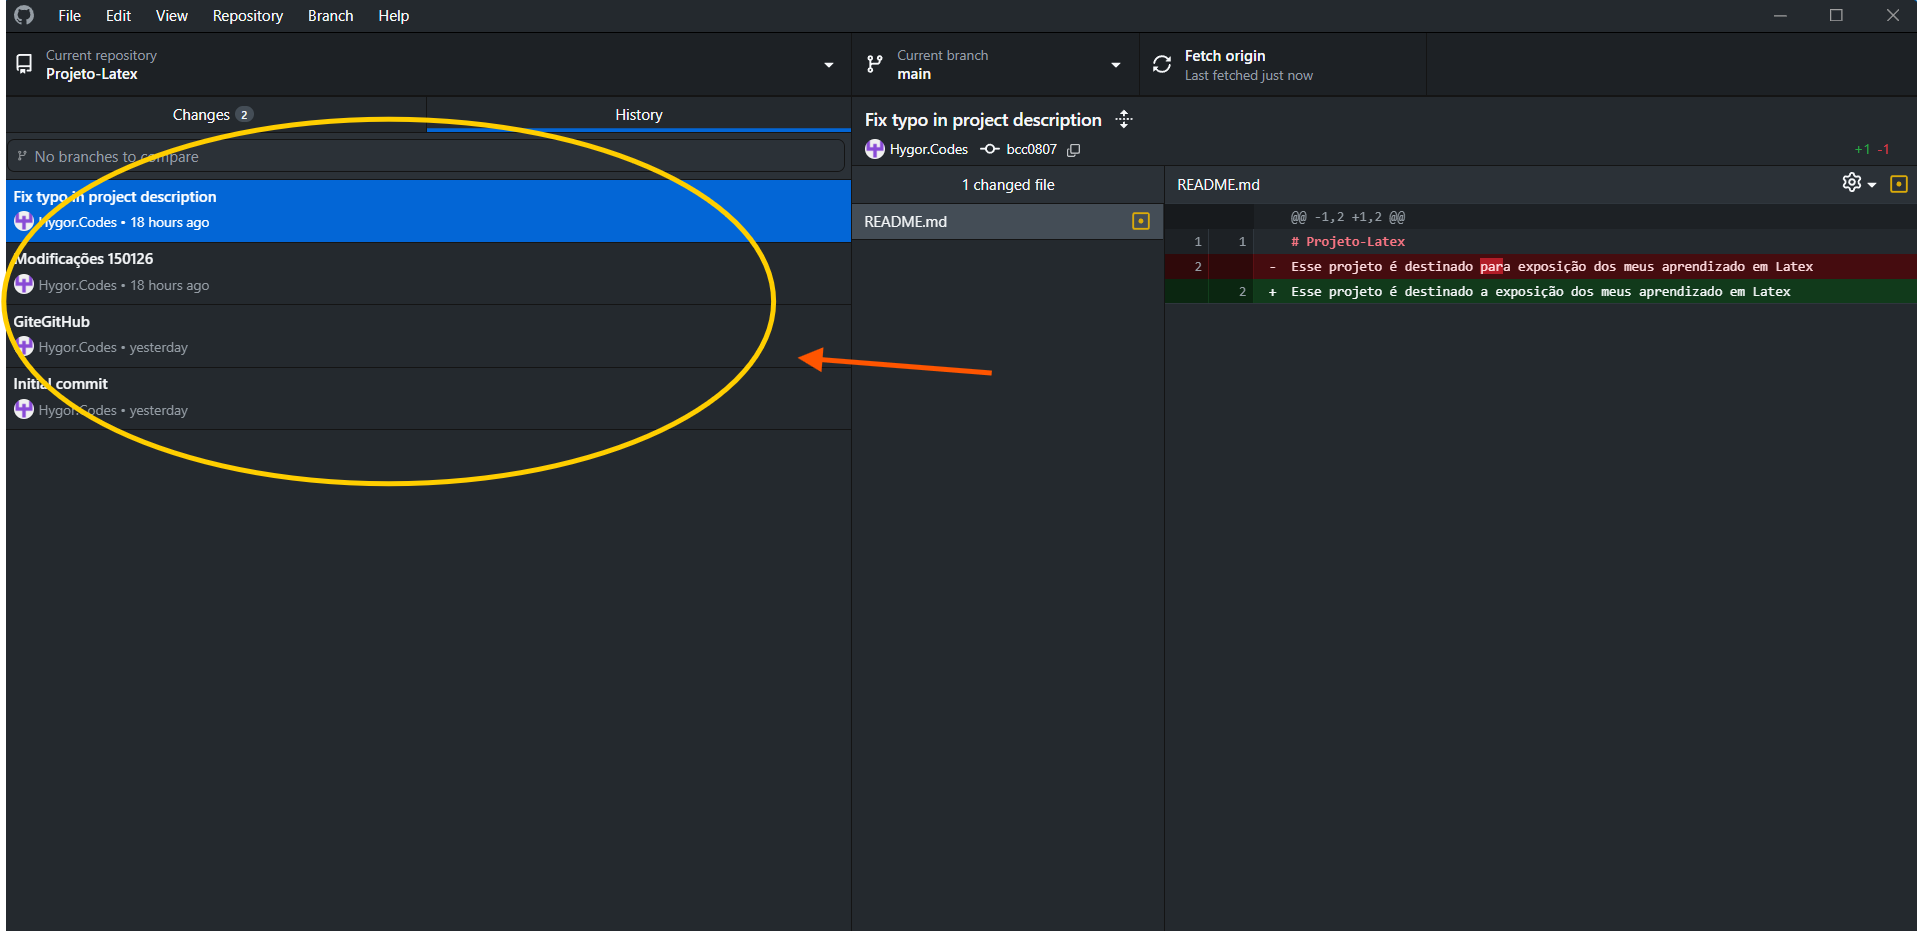
\includegraphics[scale=0.35]{./imagens/historicocommit.png}
    \end{figure}
    
    \newpage
    
    \section{Capítulo 7 $ \blacktriangleright $ Guia de Linguagem Markdown}
    
    O \textbf{MarkDown} é uma linguagem de marcação criada por criada por John Gruber e Aaron Swartz em 2004. Ela foi desenvolvida para ser uma versão simplificada do html; resumidamente. Temos varias possibilidades de aplicação mesmo para fazer diagramas. Abaixo apresento uma exposição daquilo que aprendi:
    
    \medskip
    
    \begin{minted}[breaklines, linenos, numbersep=5pt, xleftmargin=1.5em]{markdown}
        # Primeiras Explicações do que é o Markdown
        ***
        Abaixo podemos verificar uma equação matemática:
        
        $$
        \sum^{n}_{n=0} \frac{n^2+2}{n-1} = ?
        $$
        
        Dentre outras possibilidades o **Markdown** pode oferecer similaridades ao __*html*__
        
        ## Construindo Tabelas
        ***
        Podemos contruir tabelas:
        
        |Num|Nome|Aluno|
        |:---|:---:|---:|
        |01|João Guimarães|9,0|
        |02|Marta Peres|8,0|
        |03|Tobias Pétrio|6,0|
        
        ## Inserindo Imagens
        
        Podemos inserir imagens:
        
        ![Logo MarkDown](https://upload.wikimedia.org/wikipedia/commons/4/48/Markdown-mark.svg)
        
        Além disso em alguns editores é possivel usar HTML se o desejo for algo mais dimencionado como podemos ver abaixo:
        
        <img src=https://upload.wikimedia.org/wikipedia/commons/4/48/Markdown-mark.svg width =100>
        
        Obs: por algum motivo o alinhamento quebra a formatação
        
        ## Implementação de listas
        ***
        As listas númericas podem ser feitas com qualquer número seguido de ponto:
        
        1. Garoto
        2. Garota
        3. Cachorro
        1. Vira-lata
        2. Husk
        1. Homem
        2. Mulher
        
        Ou pode ser feita com asterisco ou traço para um lista não ordenada:
        
        * Hoje
        * Agora
        * Amanhã
        
        - Depois
        - Tarde
        - Postergar
        
        Pode ser também uma lista de a fazer:
        
        - [ ] Comprar água
        - [x] Comprar maçã
        - [ ] ~~Comprar suco~~
        
        Para completar uma tarefa basta inserir um X.    
    \end{minted}
    
    \section{Capítulo 8 $ \blacktriangleright $ Git Branch no GitHub-Desktop}
    
\end{document}